\documentclass[journal,hidelinks]{IEEEtran}
\usepackage[utf8]{inputenc}
\usepackage[
  pdftitle={Assignment \#3},
  pdfauthor={Andrei Purcarus},
  pdfsubject={ECSE-543 -- Numerical Methods in EE}
]{hyperref}
\usepackage{graphicx}
\usepackage[all]{hypcap}
\usepackage{amsmath}
\usepackage{amssymb}
\usepackage{cleveref}
\usepackage{indentfirst}
\usepackage[per-mode=symbol]{siunitx}
\usepackage{listings}
\lstset{showstringspaces=false}

\title{ECSE-543 \\ Numerical Methods in EE \\ Assignment \#3}
\author{Andrei~Purcarus,~260631911,~\IEEEmembership{McGill~University}}

\begin{document}
\sloppy

\maketitle

\section*{Code Listings and Unit Testing}

The source code used for this assignment is listed in the appendices. In order to save space, we did not include the unit tests. For the full code, see the \href{https://github.com/Gripnook/ECSE543-F17-A3}{GitHub repository}.

\Cref{sec:main} defines the main function, which contains the core code that produces answers to the questions in this assignment. \Cref{sec:polynomial-h,sec:polynomial-cpp} define a polynomial class. \Cref{sec:interpolation-h,sec:interpolation-cpp} define functions that perform interpolation on data. \Cref{sec:solver-h,sec:solver-cpp} define nonlinear equation solvers. \Cref{sec:matrix} defines a matrix library. \Cref{sec:cholesky} defines functions that perform Cholesky decomposition using banded and non-banded methods. \Cref{sec:matrix-solver} defines a generic solver for systems of equations that have a positive-definite coefficient matrix. Finally, \Cref{sec:integral-h,sec:integral-cpp} define functions that perform numerical integration.

\section*{Question 1}

\subsection*{(a)}

We started by performing interpolation on the first $6$ points in the B-H data for M19 steel using a Lagrange polynomial on the entire domain. To do this, we used the Lagrange interpolation function defined in \Cref{sec:interpolation-h,sec:interpolation-cpp}. The result is shown in \Cref{fig:q1a}. From this figure, we can see that the interpolated curve matches the data well over this range, since it is monotonically increasing and does not have any significant ``wiggles''.

\begin{figure}[!htb]
  \centering
  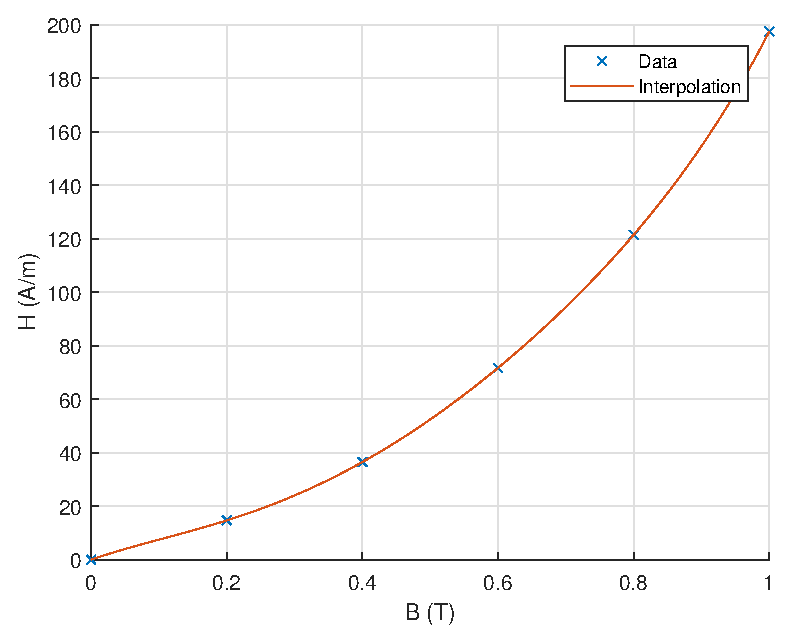
\includegraphics[width=\columnwidth]{question-1/q1a.eps}
  \caption{A Lagrange interpolation of the first $6$ points in the B-H data for M19 steel.}
  \label{fig:q1a}
\end{figure}

\subsection*{(b)}

Next, we performed the same Lagrange polynomial interpolation on the $6$ points at $B = \SI{0.0}{\tesla}$, $B = \SI{1.3}{\tesla}$, $B = \SI{1.4}{\tesla}$, $B = \SI{1.7}{\tesla}$, $B = \SI{1.8}{\tesla}$, and $B = \SI{1.9}{\tesla}$.  The results are shown in \Cref{fig:q1b}. From this figure, we can see that the result matches the data well for $B \ge \SI{1.3}{\tesla}$, but has a large deviation between $B = \SI{0.0}{\tesla}$ and $B = \SI{1.3}{\tesla}$ that does not seem plausible for the given data. This is likely to have occurred due to the lack of data in the latter range, as well as the high order polynomial we used to perform the interpolation.

\begin{figure}[!htb]
  \centering
  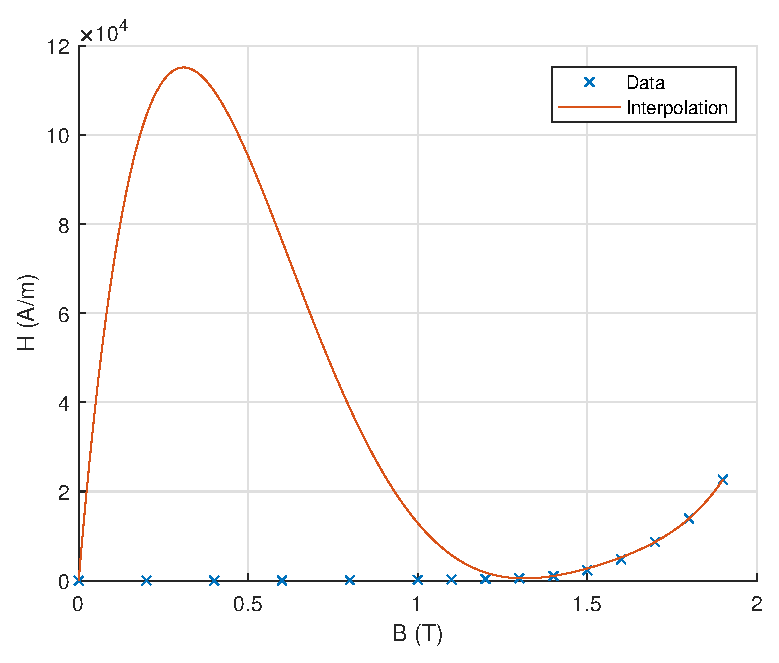
\includegraphics[width=\columnwidth]{question-1/q1b.eps}
  \caption{A Lagrange interpolation of the $6$ points at $B = \SI{0.0}{\tesla}$, $B = \SI{1.3}{\tesla}$, $B = \SI{1.4}{\tesla}$, $B = \SI{1.7}{\tesla}$, $B = \SI{1.8}{\tesla}$, and $B = \SI{1.9}{\tesla}$ in the B-H data for M19 steel.}
  \label{fig:q1b}
\end{figure}

\subsection*{(c)}

As an alternative to full-domain Lagrange interpolation, we also used cubic Hermite interpolation on each of the $5$ sub-domains between the $6$ points used in the previous section. To do this, we used the Hermite interpolation function shown in \Cref{sec:interpolation-h,sec:interpolation-cpp}. However, to do this, we had to provide values for the derivatives of the function at the given points. The simplest approach to this is to provide a numerical estimate of the derivative using the given data. Therefore, we used the slope between the points immediately before and after a given point to estimate the derivative at that point. For $B = \SI{0.0}{\tesla}$ and $B = \SI{1.9}{\tesla}$, we instead used a one-sided estimate of the derivative since points were not available on both sides. The results of doing this are shown in \Cref{fig:q1c}. From this figure, we can see that the interpolation is better than the one using Lagrange polynomials. However, it still has some problems. Due to the large gap in data, the curve initially decreases below $\SI{0.0}{\ampere\per\meter}$, which is not a realistic scenario.

\begin{figure}[!htb]
  \centering
  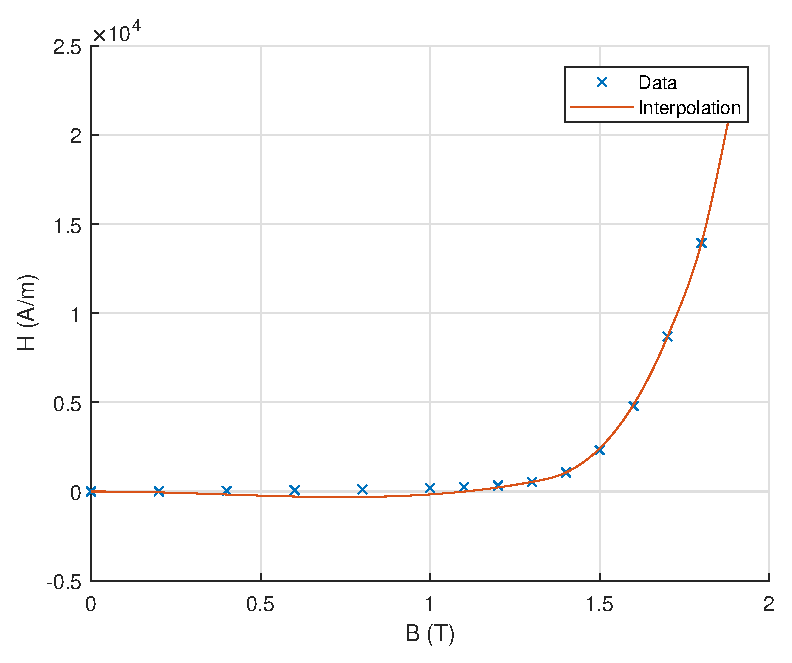
\includegraphics[width=\columnwidth]{question-1/q1c.eps}
  \caption{A piecewise cubic Hermite interpolation of the $6$ points at $B = \SI{0.0}{\tesla}$, $B = \SI{1.3}{\tesla}$, $B = \SI{1.4}{\tesla}$, $B = \SI{1.7}{\tesla}$, $B = \SI{1.8}{\tesla}$, and $B = \SI{1.9}{\tesla}$ in the B-H data for M19 steel.}
  \label{fig:q1c}
\end{figure}

\section*{Question 2}

\subsection*{(a)}

We started by deriving an equation for the flux $\Psi$ in the magnetic circuit. From Ampere's law, we have
\begin{equation}
N I = H_c l_c + H_g l_g
\end{equation}
Since the cross-sectional area $S$ is uniform in the solenoid, so are the magnetic flux $\Psi$ and the magnetic flux density $B$. Given that $H_c$ depends on $B$ according to the non-linear M19 steel data, and that $H_g$ depends on $B$ in a linear fashion, we can write
\begin{align}
N I &= H_c(B) l_c + B l_g / \mu_0 \\
N I &= H_c(\Psi / S) l_c + \Psi l_g / (\mu_0 S)
\end{align}
Thus, the equation to solve is $f(\Psi) = 0$, where
\begin{align}
f(\Psi) &= H_c(\Psi / S) l_c + \Psi l_g / (\mu_0 S) - N I \\
f'(\Psi) &= H_c'(\Psi / S) l_c / S + l_g / (\mu_0 S)
\end{align}

\subsection*{(b)}

With the equations derived in the previous section, we used the Newton-Raphson method to solve for the flux $\Psi$. The code that does this is shown in \Cref{sec:solver-h,sec:solver-cpp}. We used a piecewise linear interpolation for $H_c(B)$ and $H_c'(B)$. We then started the solver with $\Psi = \SI{0.0}{\tesla\meter^2}$ and stopped when $|f(\Psi) / f(0)| < 10^{-6}$. The resulting output of the program is shown in \Cref{fig:q2b}, which shows that the final result was $\Psi = \SI{0.000161269}{\tesla\meter^2}$, corresponding to a flux density of $B = \SI{1.61269}{\tesla}$. The figure also shows that convergence took only $3$ iterations.

\begin{figure}[!htb]
  \centering
  \includegraphics[width=0.8\columnwidth]{question-2/q2b.png}
  \caption{The output of the program for the magnetic circuit solver using the Newton-Raphson method.}
  \label{fig:q2b}
\end{figure}

\subsection*{(c)}

We next tried solving the same magnetic circuit using successive substitution. We first modified the equation to be in the form $\Psi = f(\Psi)$, as
\begin{align}
\Psi l_g / (\mu_0 S) &= N I - H_c(\Psi / S) l_c \\
\Psi &= \mu_0 S / l_g (N I - H_c(\Psi / S) l_c)
\end{align}

We tried using the successive substitution solver shown in \Cref{sec:solver-h,sec:solver-cpp}, but the problem failed to converge to a solution. In order to make the problem converge, we performed an inversion of the given equation, as
\begin{align}
H_c(\Psi / S) l_c &= N I - \Psi l_g / (\mu_0 S) \\
H_c(\Psi / S) &= (N I - \Psi l_g / (\mu_0 S)) / l_c \\
\Psi &= S H_c^{-1}((N I - \Psi l_g / (\mu_0 S)) / l_c)
\end{align}

This reformulation of the problem did converge using successive substitution, and the results are shown in \Cref{fig:q2c}. This figure shows that the solver converged to the same solution of $\Psi = \SI{0.000161269}{\tesla\meter^2}$, but said convergence was a lot slower, taking $14$ iterations.

\begin{figure}[!htb]
  \centering
  \includegraphics[width=0.8\columnwidth]{question-2/q2c.png}
  \caption{The output of the program for the magnetic circuit solver using the successive substitution method.}
  \label{fig:q2c}
\end{figure}

\section*{Question 3}

\subsection*{(a)}

We next attempted to solve the non-linear electric circuit shown in \Cref{fig:q3-circuit} by using a node voltage method to derive a system of equations. We defined the node voltages $v_1$ and $v_2$ as shown in the figure, and derived the system $\boldsymbol{f}(\boldsymbol{v}) = \boldsymbol{0}$, where
\begin{align}
\boldsymbol{f}(\boldsymbol{v}) &=
\begin{bmatrix}
(v_1 - E) / R + I_{sA} (e^{(v_1 - v_2)/v_t} - 1) \\
-I_{sA} (e^{(v_1 - v_2)/v_t} - 1) + I_{sB} (e^{v_2/v_t} - 1) \\
\end{bmatrix}
\end{align}
Note that we used $v_t = kT/q = \SI{25}{\milli\volt}$.

\begin{figure}[!htb]
  \centering
  \includegraphics[width=0.5\columnwidth]{question-3/q3-circuit.pdf}
  \caption{The non-linear electric circuit used in Question 3.}
  \label{fig:q3-circuit}
\end{figure}

\subsection*{(b)}

In order to solve the system of equations using the Newton-Raphson method, we also derived a formula for the Jacobian of $\boldsymbol{f}$ as
\begin{align}
\boldsymbol{J}(\boldsymbol{v}) &=
\begin{bmatrix}
\partial f_1 / \partial v_1 & \partial f_1 / \partial v_2 \\
\partial f_2 / \partial v_1 & \partial f_2 / \partial v_2 \\
\end{bmatrix}
\end{align}
where
\begin{align}
\partial f_1 / \partial v_1 &= 1 / R + I_{sA} e^{(v_1 - v_2)/v_t} / v_t \\
\partial f_1 / \partial v_2 &= -I_{sA} e^{(v_1 - v_2)/v_t} / v_t \\
\partial f_2 / \partial v_1 &= -I_{sA} e^{(v_1 - v_2)/v_t} / v_t \\
\partial f_2 / \partial v_2 &= I_{sA} e^{(v_1 - v_2)/v_t} / v_t + I_{sB} e^{v_2/v_t} / v_t
\end{align}

Since this Jacobian is positive definite, we used the Cholesky decomposition based solver we implemented in Assignment \#1 to solve the update equation given by
\begin{align}
\boldsymbol{J}(\boldsymbol{v}^{k}) \boldsymbol{v}^{k+1} = \boldsymbol{J}(\boldsymbol{v}^{k}) \boldsymbol{v}^{k} - \boldsymbol{f}(\boldsymbol{v}^{k})
\end{align}
The code that does this is shown in \Cref{sec:matrix-solver}. In addition, the Newton-Raphson solver for matrix equations is shown in \Cref{sec:solver-h,sec:solver-cpp}. We defined the error $\epsilon_k$ at each iteration as $\epsilon_k = \sum_{i} |f_i(\boldsymbol{v}^{k})| / \sum_{i} |f_i(\boldsymbol{v}^{0})|$, and stopped when $\epsilon_k < 10^{-6}$.

The results of the solver are shown in \Cref{fig:q3-voltages,fig:q3-residual,fig:q3-error,fig:q3-error-ratio}. In \Cref{fig:q3-voltages}, we can see that the voltages across the diodes converged to values of $V_A = \SI{0.1075633}{\volt}$ and $V_B = \SI{0.0905707}{\volt}$ in only $6$ iterations. \Cref{fig:q3-residual} shows the values of the function $\boldsymbol{f}$ across these $6$ iterations. Finally, \Cref{fig:q3-error} shows the error for each iteration.

In order to evaluate if the convergence was quadratic, we plotted $\epsilon_k / \epsilon_{k-1}^2$ in \Cref{fig:q3-error-ratio}. This figure shows that starting with iteration $2$, this ratio tended asymptotically towards a constant value. This indicates that the convergence is indeed quadratic after a few iterations. Unfortunately, the convergence of the function was so quick that we could not observe the effect in more detail.

\begin{figure}[!htb]
  \centering
  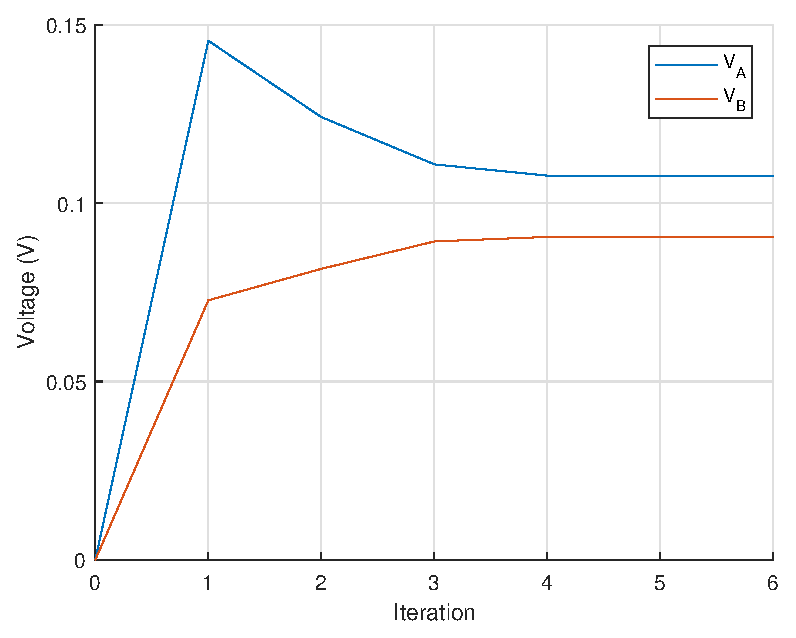
\includegraphics[width=\columnwidth]{question-3/voltages.eps}
  \caption{Diode voltages vs. iteration for the Newton-Raphson solver used to solve the circuit in \Cref{fig:q3-circuit}.}
  \label{fig:q3-voltages}
\end{figure}

\begin{figure}[!htb]
  \centering
  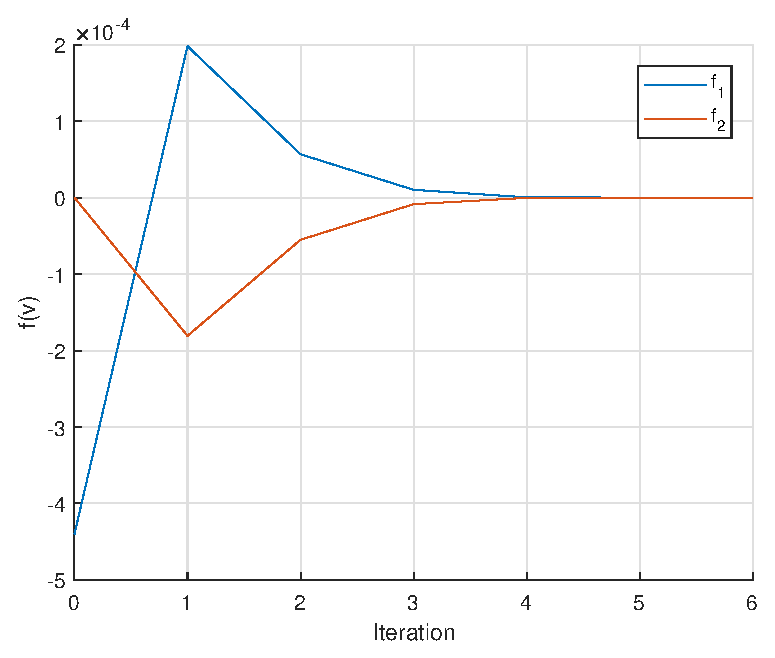
\includegraphics[width=\columnwidth]{question-3/residual.eps}
  \caption{Residual vs. iteration for the Newton-Raphson solver used to solve the circuit in \Cref{fig:q3-circuit}.}
  \label{fig:q3-residual}
\end{figure}

\begin{figure}[!htb]
  \centering
  \includegraphics[width=\columnwidth]{question-3/error.eps}
  \caption{Error vs. iteration for the Newton-Raphson solver used to solve the circuit in \Cref{fig:q3-circuit}.}
  \label{fig:q3-error}
\end{figure}

\begin{figure}[!htb]
  \centering
  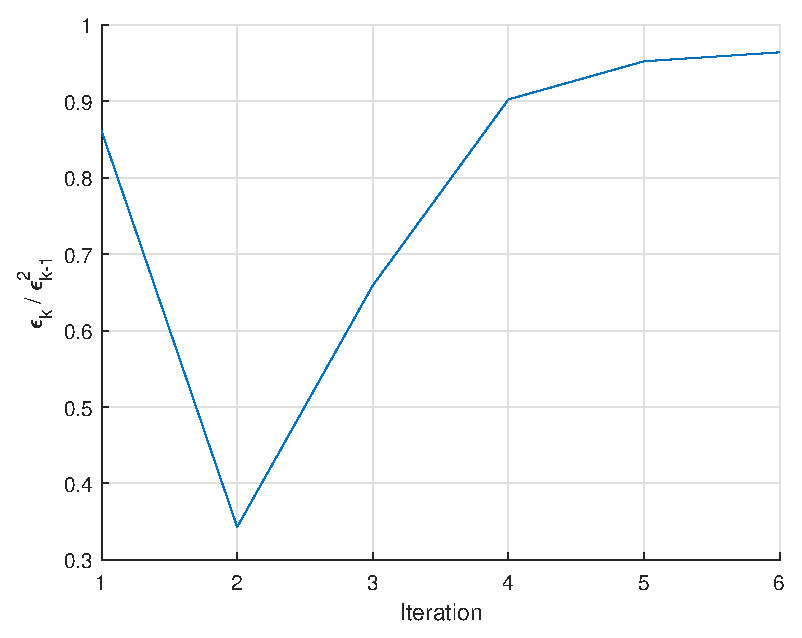
\includegraphics[width=\columnwidth]{question-3/error_ratio.eps}
  \caption{Error ratio vs. iteration for the Newton-Raphson solver used to solve the circuit in \Cref{fig:q3-circuit}.}
  \label{fig:q3-error-ratio}
\end{figure}

\section*{Question 4}
\subsection*{(a)}

Next, we performed numerical integration on the function $f(x) = cos(x)$ from $x = 0$ to $x = 1$ using one-point Gauss-Legendre integration over $N$ equal segments. The code that performs this function is shown in \Cref{sec:integral-h,sec:integral-cpp}. The results are shown in \Cref{fig:q4a}, which shows the natural logarithm of the absolute error plotted against the natural logarithm of the number of segments. This figure shows a clear linear trend, with a mean slope of $-2.0031$. This indicates that the error is approximately proportional to $1/N^2$, as we would expect since the one-point method integrates linear functions exactly and thus the error should be quadratic.

\begin{figure}[!htb]
  \centering
  \includegraphics[width=\columnwidth]{question-4/q4a.eps}
  \caption{$ln(E)$ vs. $ln(N)$ for the integral of $f(x) = cos(x)$ from $x = 0$ to $x = 1$ using one-point Gauss-Legendre integration over $N$ equal segments.}
  \label{fig:q4a}
\end{figure}

\subsection*{(b)}

Next, we applied the same method to the function $f(x) = ln(x)$ from $x = 0$ to $x = 1$. The results are shown in \Cref{fig:q4b}, which shows the natural logarithm of the absolute error plotted against the natural logarithm of the number of segments. This figure shows a clear linear trend, with a mean slope of $-0.9981$. This indicates that the error is approximately proportional to $1/N$. Thus the error for this function has a lower order than for $f(x) = cos(x)$. This can be explained by the fact that $f(x) = ln(x)$ is unbounded on the integration interval. Indeed, since the second derivative tends to $-\infty$ as $x \to 0$, we cannot use a simple Taylor series to show that the error should be quadratic on this interval.

\begin{figure}[!htb]
  \centering
  \includegraphics[width=\columnwidth]{question-4/q4b.eps}
  \caption{$ln(E)$ vs. $ln(N)$ for the integral of $f(x) = ln(x)$ from $x = 0$ to $x = 1$ using one-point Gauss-Legendre integration over $N$ equal segments.}
  \label{fig:q4b}
\end{figure}

\subsection*{(c)}

Finally, we attempted to integrate the function $f(x) = ln(x)$ as accurately as possible using a one-point Gauss-Legendre method with only $10$ segments. We wrote a function that accepts a vector of segment lengths and performs this computation. The code for this is shown in \Cref{sec:integral-h,sec:integral-cpp}.

In order to perform a methodical study, we decided to divide the lengths according to a geometric ratio, which would make the segments close to the singularity at $x = 0$ shorter compared to the segments close to $x = 1$. Thus, we used segments of the form $\alpha$, $\alpha r$, $\ldots$, $\alpha r^9$. We varied $r$ from $1$ to $2$ and computed $\alpha$ using
\begin{align}
\alpha (1 + r + ... + r^{9}) &= 1 \\
\alpha (r^{10} - 1) / (r - 1) &= 1 \\
\alpha &= (r - 1) / (r^{10} - 1)
\end{align}

The results of this approach are shown in \Cref{fig:q4c}. This figure shows that the error reaches a minimum of $0.0106114$ at $r = 1.45$, which corresponds to $\alpha = 0.0112262$.

\begin{figure}[!htb]
  \centering
  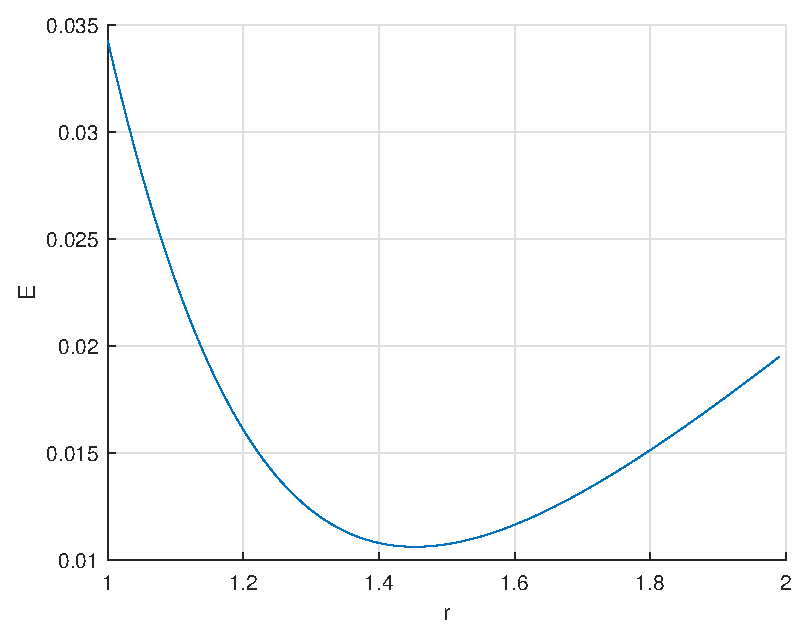
\includegraphics[width=\columnwidth]{question-4/q4c.eps}
  \caption{$E$ vs. $r$ for the integral of $f(x) = ln(x)$ from $x = 0$ to $x = 1$ using one-point Gauss-Legendre integration over $10$ unequal segments.}
  \label{fig:q4c}
\end{figure}

\newpage
\onecolumn

\begin{appendices}

\section{Main.cpp}
\label{sec:main}
\lstinputlisting[language=C++]{src/main.cpp}
\newpage

\section{Polynomial.h}
\label{sec:polynomial-h}
\lstinputlisting[language=C++]{src/polynomial.h}
\newpage

\section{Polynomial.cpp}
\label{sec:polynomial-cpp}
\lstinputlisting[language=C++]{src/polynomial.cpp}
\newpage

\section{Interpolation.h}
\label{sec:interpolation-h}
\lstinputlisting[language=C++]{src/interpolation.h}
\newpage

\section{Interpolation.cpp}
\label{sec:interpolation-cpp}
\lstinputlisting[language=C++]{src/interpolation.cpp}
\newpage

\section{Solver.h}
\label{sec:solver-h}
\lstinputlisting[language=C++]{src/solver.h}
\newpage

\section{Solver.cpp}
\label{sec:solver-cpp}
\lstinputlisting[language=C++]{src/solver.cpp}
\newpage

\section{Matrix.h}
\label{sec:matrix}
\lstinputlisting[language=C++]{src/matrix.h}
\newpage

\section{Cholesky.h}
\label{sec:cholesky}
\lstinputlisting[language=C++]{src/cholesky.h}
\newpage

\section{Matrix-solver.h}
\label{sec:matrix-solver}
\lstinputlisting[language=C++]{src/matrix-solver.h}
\newpage

\section{Integral.h}
\label{sec:integral-h}
\lstinputlisting[language=C++]{src/integral.h}
\newpage

\section{Integral.cpp}
\label{sec:integral-cpp}
\lstinputlisting[language=C++]{src/integral.cpp}
\newpage

\end{appendices}

\end{document}
